\chapter{Antecedentes}
\label{chap:antecedentes}

\drop{E}{n} este capítulo se expondrán unos conocimientos básicos para poder comprender mejor este documento. Se presentarán 
los tipos de aplicaciones para móviles que se desarrollan hoy en día y se mostrarán algunas de las aplicaciones para móviles
de la competencia directa de Nextinit.

\section{Tipos de aplicaciones móviles}

Antes de ver los tipos de aplicaciones móviles que existen, es necesario conocer que es una aplicación móvil. Las aplicaciones
móviles o simplemente apps son aplicaciones informáticas que diseñadas para ser ejecutadas en dispositivos móviles, tales 
como smartphones y tablets.

Actualmente, se pueden desarrollar aplicaciones móviles de distintas formas \cite{ANADES} como se verá a continuación, el 
principal reto de los desarrolladores es proporcionar soluciones para todas las plataformas.  A continuación se presentarán 
tres tipos de aplicaciones, una mediante un desarrollo por plataforma (nativa) y dos multiplataforma (híbrida y web), en 
función de las necesidades será recomendable usar un tipo u otro.

\subsection{Aplicaciones nativas}

Las aplicaciones nativas se desarrollan para un \acf{SO} determinado. En cada \acs{SO} se utiliza un lenguaje y entorno 
específico para desarrollar en esa plataforma siendo compilada para funcionar únicamente en esta, lo que, generalmente 
permite un funcionamiento más fluido y estable que otro tipo de aplicaciones.

La principal ventaja de las aplicaciones nativas es la posibilidad de acceder a todos los elementos del dispositivo móvil, tales
como el \acs{GPS} o la cámara. Por el contrario, el problema más notable es el coste de desarrollo, ya que es necesario
un desarrollo distinto por cada \acs{SO} en el que se quiera disponer de la aplicación (ver Cuadro~\ref{tab:nativas}).

\begin{table}[nativas]
	\centering
	{\small
		


\begin{tabular}{p{.2\textwidth}p{.2\textwidth}}
  \tabheadformat
  \tabhead{Ventajas}   &
  \tabhead{Inconvenientes}           \\
\hline
    & Acceso completo a los recursos del dispositivo						   & Diferentes lenguajes y entornos para cada plataforma \\
					& Mejor experiencia de usuario									& Tienden a ser más caras de desarrollar \\
					& Envío de notificaciones push   & El código del cliente no es reutilizable entre las diferentes plataformas \\
					& Se pueden añadir aves de las tiendas de aplicaciones

\hline
\end{tabular}


% Local variables:
%   coding: utf-8
%   ispell-local-dictionary: "castellano8"
%   TeX-master: "main.tex"
% End:

	}
	\caption[Ventajas e inconvenientes de las aplicaciones móviles nativas]
	{Ventajas e inconvenientes de las aplicaciones móviles nativas~\cite{TIPAPP}}
	\label{tab:nativas}
\end{table}

\subsection{Aplicaciones web}
Las aplicaciones web para móviles son ejecutadas desde un navegador web del dispositivo. Estas aplicaciones se desarrollan
como si fuera una web, con las mismas tecnologías. Por ese motivo, este tipo de aplicaciones no necesitan la instalación 
de ningún componente para utilizar la aplicación, únicamente necesitan un navegador y conexión a Internet. 

Además, como no se instala nada en el dispositivo, las actualizaciones son aplicadas únicamente en el servidor, con lo cuál, 
los usuarios siempre usan la última actualización disponible, sin que el usuario tenga que actualizar ningún componente 
en dicho dispositivo.

La gran ventaja es la independencia del \acs{SO} a la hora de desarrollar la aplicación, con el mismo desarrollo se consigue 
una solución capaz de ejecutarse en cualquiera de ellos que disponga de un navegador web y conexión a Internet. 

Pero, como se ha comentado anteriormente estas aplicaciones dependen totalmente de una conexión a Internet para 
funcionar, y aún teniendo conexión si esta no es estable puede ofrecer una experiencia de usuario bastante negativa. A 
parte de la dependencia de la conexión presenta otros problemas como la imposibilidad de utilizar todos los elementos 
del dispositivo como el \acs{GPS} o el bluetooth (ver Cuadro~\ref{tab:web}).

\begin{table}[web]
	\centering
	{\small
		


\begin{tabular}{p{.4\textwidth}p{.4\textwidth}}
	\tabheadformat
	\tabhead{Ventajas}   &
	\tabhead{Inconvenientes}      \\
	\hline
	 & Es multiplataforma							   & Diferentes habilidades / idiomas / herramientas para cada plataforma \\
	& El desarrollo es más sencillo y económico								& Tienden a ser más caras de desarrollar \\
	& El usuario siempre dispone de la última versión   & El código del cliente no es reutilizable entre las diferentes plataformas \\
	
	\hline
\end{tabular}


% Local variables:
%   coding: utf-8
%   ispell-local-dictionary: "castellano8"
%   TeX-master: "main.tex"
% End:

	}
	\caption[Ventajas e inconvenientes de las aplicaciones web móviles]
	{Ventajas e inconvenientes de las aplicaciones web móviles~\cite{TIPAPP}}
	\label{tab:web}
\end{table}

\subsection{Aplicaciones híbridas}

Las aplicaciones híbridas combinan parte de las características los dos tipos anteriores. Se utilizan tecnologías web 
como puede ser Javascript o HTML, utilizando el mismo código para distintas plataformas. Pero además, pueden 
acceder a parte de los elementos hardware del dispositivo, aunque no se tiene un control total de este como 
ocurría en las nativas. Otra de las características es la necesidad de instalar la aplicación en los dispositivos, por 
lo que se pueden distribuir a través de las tiendas de aplicaciones.

En cambio, una de las desventajas es que al hacer un solo desarrollo, el diseño de la interfaz de usuario será igual
en cualquiera de las plataformas pudiendo no adaptarse a los estilos de estas (ver Cuadro~\ref{tab:hibridas}). Aunque, esto puede solucionarse
habría que añadir código específico para cada \acs{SO} para que la aplicación se adapte.

\begin{table}[hibridas]
	\centering
	{\small
		


\begin{tabular}{p{.4\textwidth}p{.4\textwidth}}
	\tabheadformat
	\tabhead{Ventajas}   &
	\tabhead{Inconvenientes}      \\
	\hline
	Se pueden distribuir a través de las tiendas de aplicaciones & Experiencia de usuario peor que una nativa \\
	Se instala en el dispositivo pero utiliza tecnologías web como Javascript o HTML & El diseño visual puede no ser acorde con el \acs{SO} \\
	Código base común para distintos \acs{SO}  & \\
	Acceso a parte de los elementos del dispositivos & \\
	
	\hline
\end{tabular}


% Local variables:
%   coding: utf-8
%   ispell-local-dictionary: "castellano8"
%   TeX-master: "main.tex"
% End:

	}
	\caption[Ventajas e inconvenientes de las aplicaciones móviles híbridas]
	{Ventajas e inconvenientes de las aplicaciones móviles híbridas~\cite{TIPAPP}}
	\label{tab:hibridas}
\end{table}

\section{Frameworks para desarrollar aplicaciones híbridas}

\subsection{Ionic Framework}

Ionic Framework~\cite{IONIC} es un SDK que permite desarrollar aplicaciones móviles de calidad y con buen 
rendimiento utilizando tecnologías web (HTML, CSS y Javascript). Ionic se centra principalmente en la apariencia 
visual y la interacción del usuario con la aplicación. 

Ionic está desarrollado sobre el framework Angular, por lo que se podrá crear código más rápido y optimizado 
explotando las características que ofrece este framework.

Además de en Angular, Ionic se basa también en Apache Cordova para construir la aplicación móvil. Mediante sus 
librerías se puede acceder a elementos del dispositivo, tales como la cámara o el \acs{GPS}.

En la Figura~\ref{fig:CORDOVAimg} se puede apreciar como Cordova hace de puente entre el WebKit y la parte nativa del sistema, y usando 
frameworks visuales como Ionic podemos simplificar el proceso de diseño.

\begin{figure}[!h]
	\begin{center}
		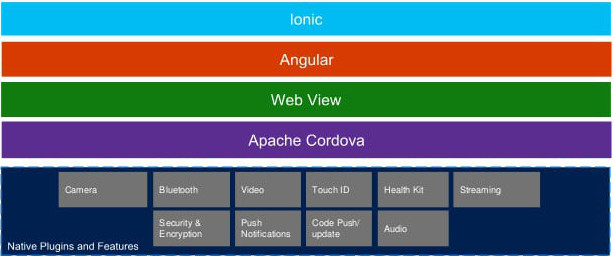
\includegraphics[width=0.8\textwidth]{./img/cordova.jpg}
		\caption{Arquitectura Ionic~\cite{CORDOVAimg}}
		\label{fig:CORDOVAimg}
	\end{center}
\end{figure}

\subsection{React Native}

React Native es un framework desarrollado por Facebook que permite desarrollar aplicaciones para Android e IOS 
con componentes nativos y un rendimiento casi al nivel de las nativas usando React. Con React Native no se crea 
una aplicación híbrida clásica sino que construye aplicaciones nativas con componentes nativos de cada \acs{SO}, 
a esto, muchos lo consideran un nuevo tipo llamado aplicaciones \acf{JIT} en vez de híbridas.

Algunas de las características~\cite{rnCaracteristicas} destacables de React Native son:
\begin{itemize}
	\item No es un WebView como Ionic sino que traduce los componentes en Javascript a componentes nativos.
	\item Al no ser una aplicación web ni estar en HTML no se usa CSS en ella, pero hay un conjunto de propiedades
	similares al CSS que se pueden utilizar para cambiar el diseño de los componentes.
	\item No es necesario recompilar la aplicacación para probar cambios, cada vez que se modifica el código 
	se puede ver en tiempo real esa modificación.
	\item Es posible utilizar código nativo en Java, Objective-C o Swift cuando se necesite. También es posible usar 
	Kotlin con la configuración adecuada de Gradle.
	\item Al estar escrita en Javascript, se puede utilizar en el proyecto gran parte de los módulos disponibles a través 
	de gestores de paquetes como «npm».
	\item Dispone de algunos polyfills o shims para Fetch o Sockets, entre otros.
\end{itemize}

\subsection{NativeScript}

NativeScript~\cite{NATSCR} al igual que React Native es un framework que permite con el mismo código base desarrollar aplicaciones 
Android e IOS, las interfaces de usuario se renderizan con componentes nativos de la plataforma, obteniendo unos 
resultados muy parecidos a las aplicaciones nativas.

Una de las características de NativeScript que lo diferencian de React Native es el lenguaje de desarrollo, ademas de 
usar Javascript se utiliza CSS y XML para las interfaces de usuario. Además, se puede utilizar TypeScript, Angular 2 y
Vue.js.

\subsection{Comparativa}

\begin{table}[comparativa]
	\centering
	{\small
		


\begin{tabular}{p{.25\textwidth}p{.25\textwidth}p{.25\textwidth}p{.25\textwidth}}
  \tabheadformat
  \tabhead{}   &
  \tabhead{IONIC} &
  \tabhead{React Native} &
  \tabhead{NativeScript} \\
\hline
    				Desarrollo multiplataforma &
    				Desarrollo web. Código válido en Android, IOS, Windows Phone y web &
    				Con el mismo código se desarrollan aplicaciones para Android e IOS &
    				Multiplataforma real. El mismo código base para desarrollar las aplicaciones
    				para todas las plataformas compatibles. \\
    				
    				Desarrollo y lenguajes usados &
    				Lenguajes de web (HTML, XML, CSS, ...) &
    				Similar a React con ES6. JSX con Javascript &
    				Javascript, CSS, XML, Typescript, Angular y Vue.js \\
    				
    				Rendimiento &
    				Peor que las aplicaciones nativas. Puede dar problemas
    				si se realizan muchas llamadas a código nativo & 
    				Mucho mejor que IONIC, las interacciones con el 
    				hardware son procesadas por la plataforma específica &
    				Si la conexión a internet es lenta puede dar problemas. El 
    				peso de la aplicación es mucho mas alto que los otros. Acceso
    				100\% a las APIs nativas \\
    				
    				Interfaz de usuario &
    				La misma para todas las plataformas. Sistema de gráficos y 
    				transiciones complejo de utilizar. &
    				Utiliza componentes nativos de la plataforma &
    				Utiliza componentes nativos de la plataforma \\
    				
    				Popularidad &
    				35k estrellas en GitHub &
    				67k estrellas en GitHub &
    				14k estrellas en GitHub \\
    				
    				Desarrollador &
    				Drifty &
    				Facebook &
    				Progress \\
    				 
    				Primera versión &
    				2013 &
    				2013 &
    				2014 \\ 
    				
    				Última versión estable &
    				4.0.5 &
    				0.56 &
    				4.0.1 \\
    				

\hline
\end{tabular}


% Local variables:
%   coding: utf-8
%   ispell-local-dictionary: "castellano8"
%   TeX-master: "main.tex"
% End:

	}
	\caption[Comparativa de IONIC, React Native, NativeScript]
	{Comparativa de IONIC, React Native y NativeScript~\cite{comparativaHibridas}}
	\label{tab:comparativa}
\end{table}

\section{Aplicaciones de la competencia}
\subsection{Spigit}

Es la plataforma de gestión de ideas líder en la industria que escala en la empresa para dar a conocer las mejores ideas. La plataforma Spigit está respaldada por algoritmos propios del pensamiento colectivo y una metodología comprobada que, en su conjunto, ofrece resultados comerciales finales. Sus sedes principales están en San Francisco, Londres y Sydney y está disponible en 11 idiomas.

Esta herramienta disponía de una aplicación para Android, pero ha sido recientemente retirada de la 
Play Store.

\begin{figure}[!h]
	\begin{center}
		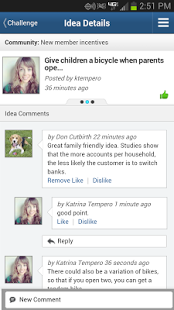
\includegraphics[width=0.2\textwidth]{./img/competencia/spigit/1.png}
		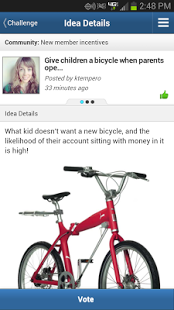
\includegraphics[width=0.2\textwidth]{./img/competencia/spigit/2.png}
		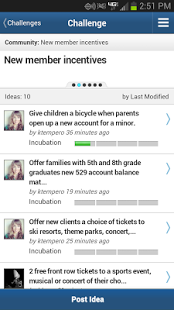
\includegraphics[width=0.2\textwidth]{./img/competencia/spigit/3.png}
		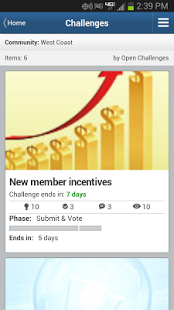
\includegraphics[width=0.2\textwidth]{./img/competencia/spigit/4.png}
		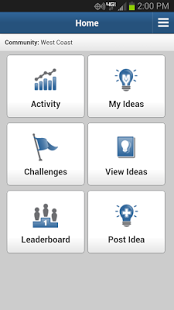
\includegraphics[width=0.2\textwidth]{./img/competencia/spigit/5.png}
		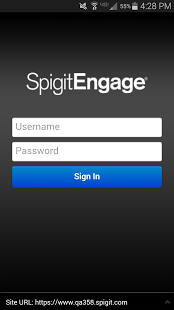
\includegraphics[width=0.2\textwidth]{./img/competencia/spigit/6.png}
		\caption{Aplicación de spigit para Android}
		\label{fig:sipigi}
	\end{center}
\end{figure}

\subsection{brightIdea}

Brightidea acelera el éxito de la innovación capacitando a quienes lo respaldan con un software avanzado para facilitar  y agilizar el proceso de ideación y la colaboración en la que se desarrolla desde 2005. Fundada en 1999, tiene entre 51 - 2000 empleados 
repartidos entre las oficinas de San Francisco y Nueva York trabaja con marcas como AXA, Cisco, Dell, GE y Motorola Solutions.

Está enfocada principalmente a medianas y grandes empresas. Dispone de aplicación para móviles como se puede ver en la figura~\ref{fig:brightIdea}

\begin{figure}[!h]
	\begin{center}
		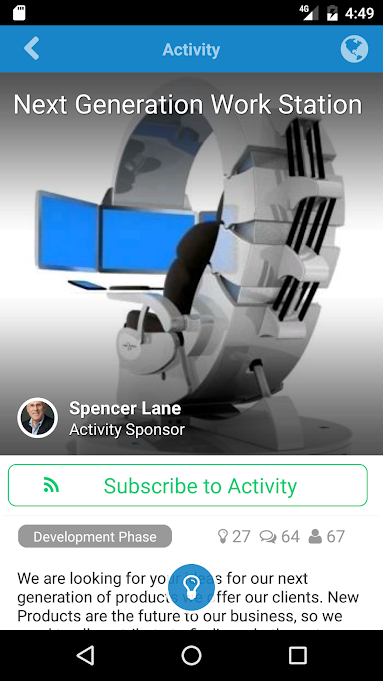
\includegraphics[width=0.2\textwidth]{./img/competencia/brightIdea/1.png}
		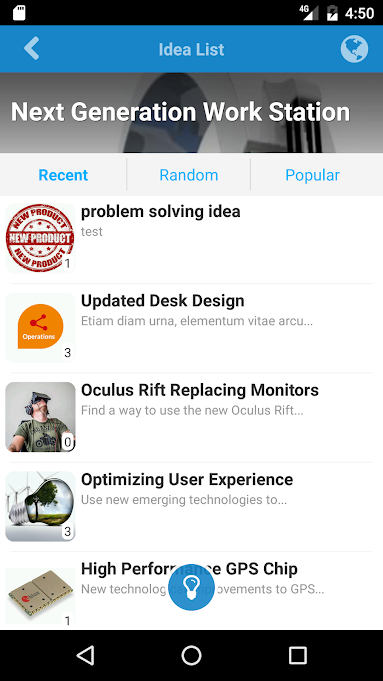
\includegraphics[width=0.2\textwidth]{./img/competencia/brightIdea/2.png}
		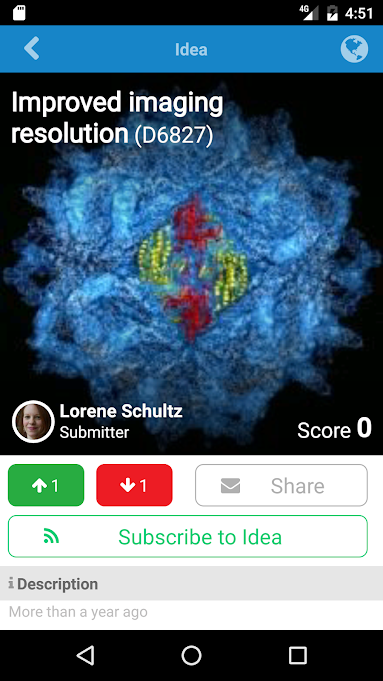
\includegraphics[width=0.2\textwidth]{./img/competencia/brightIdea/3.png}
		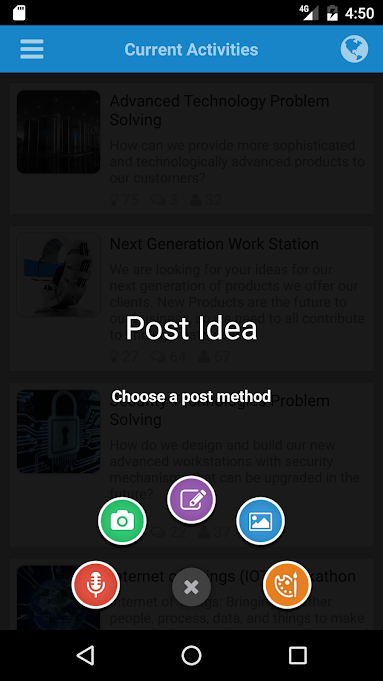
\includegraphics[width=0.2\textwidth]{./img/competencia/brightIdea/4.png}
		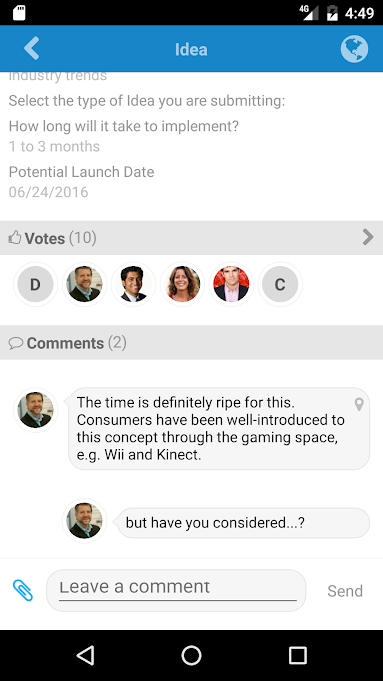
\includegraphics[width=0.2\textwidth]{./img/competencia/brightIdea/5.png}
		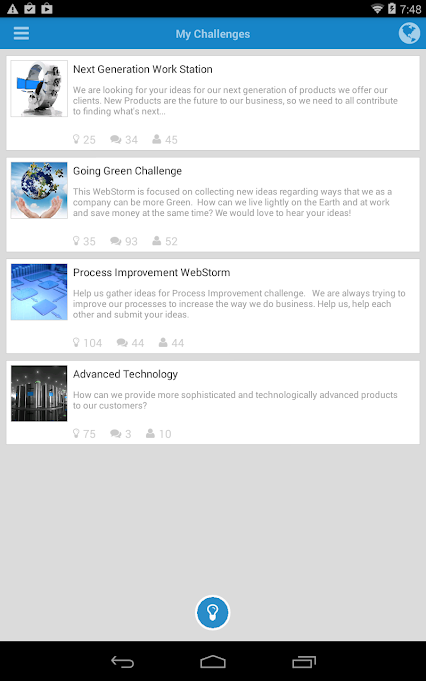
\includegraphics[width=0.2\textwidth]{./img/competencia/brightIdea/6.png}
		\caption{Aplicación de brightIdea para Android}
		\label{fig:brightIdea}
	\end{center}
\end{figure}

\subsection{ideas4all}

Es una comunidad online para personas que tienen ideas y para las que las buscan. A través de esta cada persona puede tener un espacio personal donde compartir, guardar y organizar sus propias ideas y al mismo tiempo inspirarse con las miles de ideas que han compartido otros usuarios.

Ideas4All no ofrece ninguna aplicación para móviles pero apoyan la creación de aplicaciones de terceros 
para interactuar con su comunidad.


\subsection{hypeInnovation}

Fundada en 2001, HYPE Innovation proporciona software y servicios para que los gerentes de innovaciones utilicen la inteligencia colectiva de sus empleados, clientes y socios. Ayudan a las organizaciones a generar ingresos adicionales, a ser más eficientes y a empoderar y conectar a las personas. Tiene clientes como Airbus, Toyota, Volvo, Siemens, Bosch, Roche, Fujitsu, Nokia, Zeiss y Danone.

Dispone de aplicaciones para móviles con iOS, Android, Windows Phone, y Blackberry (Ver figura~\ref{fig:hype}).

\begin{figure}[!h]
	\begin{center}
		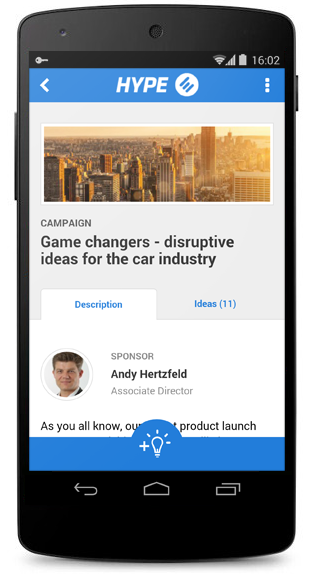
\includegraphics[width=0.2\textwidth]{./img/competencia/hype/1.png}
		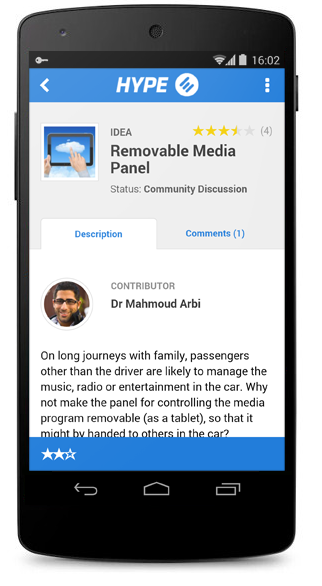
\includegraphics[width=0.2\textwidth]{./img/competencia/hype/2.png}
		\caption{Aplicación de hype para Android}
		\label{fig:hype}
	\end{center}
\end{figure}

%\subsection{exago}

%- Entre 4,5€ y 1,5€ por usuario al mes.
%- Dice tener versión de móvil.
%- 30 días de prueba
%- Analíticas de datos
%- Challenge e ideas con definiciones flexibles
%- Disponible un catalogo de recompensas para los usuarios
%- En Inglés, Francés, Italiano, Portugués, Ruso, Español
%
%
%
%\subsection{Qmarkets}
%
%- Free trial
%- Integración con SharePoint, Twitter, Linkedin, Facebook, Twiter, Yammer, Jive, Sap Digital CRM
%- Sin puntuación y sin nuevas versiones desde 2016 para IOS
%- No disponible en google play (hay apks por ahí)
%

% Local Variables:
%  coding: utf-8
%  mode: latex
%  mode: flyspell
%  ispell-local-dictionary: "castellano8"
% End:
